\section{Cambiar Contraseña}

Es importante estár cambiando regularmente una contraseña para mantener la seguridad de nuestros datos. Es por eso que se le permite al Paciente cambiar su contraseña cada que éste lo solicite.

\subsubsection{Procedimiento}
\begin{enumerate}
	
	\item Da clic en el icono \textbf{Editar Información} de la pantalla \textbf{Datos Principales}.

	\item Se mostrará la pantalla \textbf{Editar Información}.
	
	\begin{figure}[!htbp]
		\hypertarget{fig:editInfo}{\hspace{1pt}}
		\begin{center}
			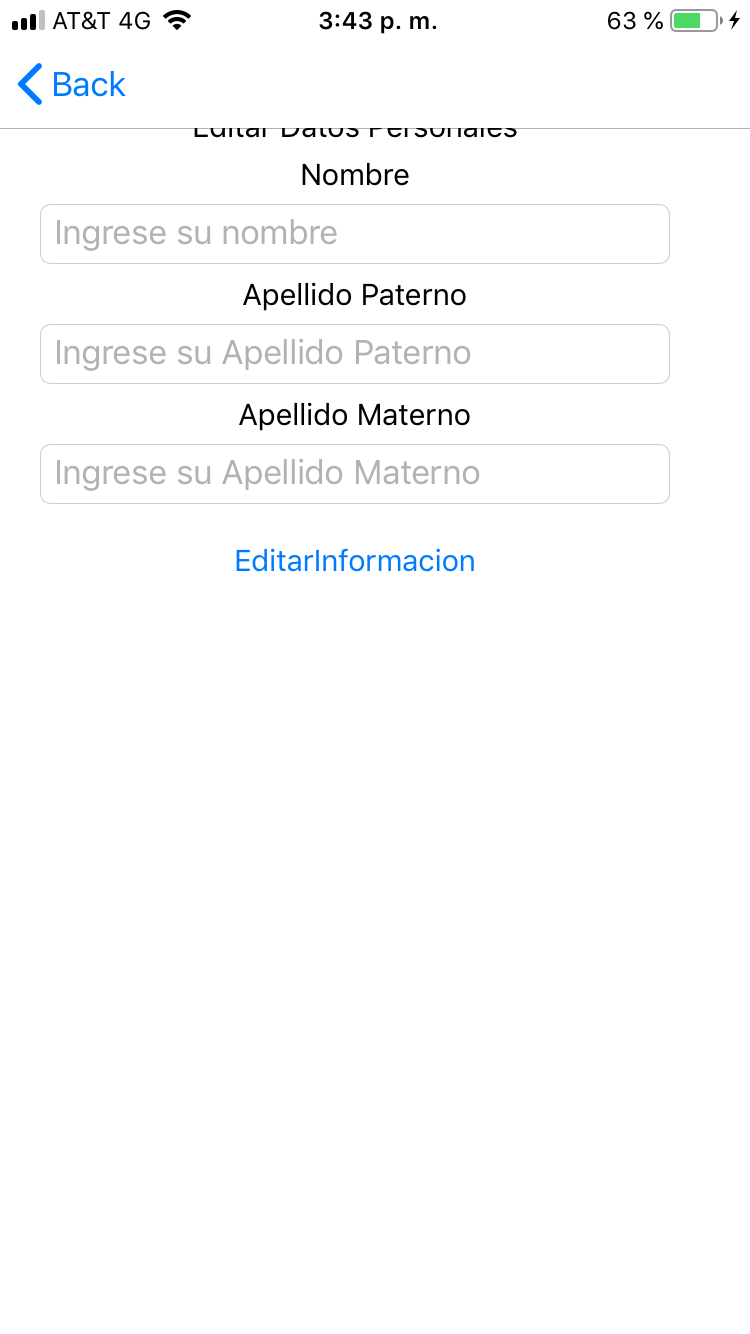
\includegraphics[height=0.4\textheight]{Paciente/CambiarContrasena/images/editInfo}
			\caption{Editar Información}
			\label{fig:editInfo}
		\end{center}
	\end{figure}

	\item Seleccione la opción\textbf{ ¿Desea editar su contraseña?} de la pantalla \textbf{Editar Información}.
	 
	\item Ingresa la nueva contraseña.
	
	\item Presiona el botón \textbf{Editar Contraseña} para guardar los cambios de tu contraseña.

\end{enumerate}

